\documentclass{article}


% if you need to pass options to natbib, use, e.g.:
%     \PassOptionsToPackage{numbers, compress}{natbib}
% before loading neurips_2023


% ready for submission
\usepackage{hypertype}


% to compile a preprint version, e.g., for submission to arXiv, add add the
% [preprint] option:
\usepackage[preprint]{neurips_2023}


% to compile a camera-ready version, add the [final] option, e.g.:
%     \usepackage[final]{neurips_2023}


% to avoid loading the natbib package, add option nonatbib:
%    \usepackage[nonatbib]{neurips_2023}


\usepackage[utf8]{inputenc} % allow utf-8 input
\usepackage[T1]{fontenc}    % use 8-bit T1 fonts
\usepackage{hyperref}       % hyperlinks
\usepackage{url}            % simple URL typesetting
\usepackage{booktabs}       % professional-quality tables
\usepackage{amsfonts}       % blackboard math symbols
\usepackage{nicefrac}       % compact symbols for 1/2, etc.
\usepackage{microtype}      % microtypography
\usepackage{xcolor}         % colors


\title{Taking Down XGBoost with CTAO}


% The \author macro works with any number of authors. There are two commands
% used to separate the names and addresses of multiple authors: \And and \AND.
%
% Using \And between authors leaves it to LaTeX to determine where to break the
% lines. Using \AND forces a line break at that point. So, if LaTeX puts 3 of 4
% authors names on the first line, and the last on the second line, try using
% \AND instead of \And before the third author name.


\author{%
  Albert Cai\\
  Department of Mechanical Engineering\\
  Stanford University\\
  \texttt{albertc4@stanford.edu} \\
  % examples of more authors
  % \And
  % Coauthor \\
  % Affiliation \\
  % Address \\
  % \texttt{email} \\
  % \AND
  % Coauthor \\
  % Affiliation \\
  % Address \\
  % \texttt{email} \\
  % \And
  % Coauthor \\
  % Affiliation \\
  % Address \\
  % \texttt{email} \\
  % \And
  % Coauthor \\
  % Affiliation \\
  % Address \\
  % \texttt{email} \\
}


\begin{document}


\maketitle


\begin{abstract}
  Since its initial release in 2014, XGBoost has become the go-to algorithm for many machine learning tasks.
  It is quick to train and its tree structure is easy to interpret. However, XGBoost has its limitations.
  Namely, (1) its greedy training structure may lead to suboptimal solutions, (2) it uses
  axis-aligned trees which may limit expressiveness, and (3) it is a
  piecewise constant predictor, which may not be the best representation of the data.
  In search of a better algorithm, we propose the convex tree alternating optimization (CTAO) algorithm, 
  a parallelized and convex implementation of the tree alternating optimization algorithm.
  Its one-iteration performance is comparable with XGBoost, while solving three times less optimization problems.
\end{abstract}


\section{Introduction}

Machine learning has become essential across various domains and decision trees are the most popular statistical models in practice.
A prediction is made by the path from the root to the leaf, each intermediate node representing a decision. 
This structure is easy to interpret and can be used for feature selection.
Today, the two most common itermediate node decisions are represented by 
axis-aligned splits ($x_j > b_i$, that is, is feature $j$ bigger than threshold $b_i$) and
oblique splits ($\mathbf{w}_i^T\mathbf{x} > b_i$, that is, a splitting hyperplane).

The core problem is that learning the best tree is computationally expensive. It is impossible to enumerate all possible tree structures.
In light of this, XGBoost, the most popular tree-based algorithm, uses a tree ensemble made up of many simpler trees. 
Its prediction is the sum of the predictions of all its trees. An illustration of XGBoost's tree ensemble is shown in Figure~\ref{xgboost-ensemble}.
Each tree uses a axis-aligned splits and a greedy algorithm to build its trees. 
Each of its trees start from a root node and inductively splits the nodes by searching over many thresholds for all features. To further
reduce the search space, its leaves are constant predictors, meaning that XGBoost is a piecewise constant predictor.

\begin{figure}
  \centering
  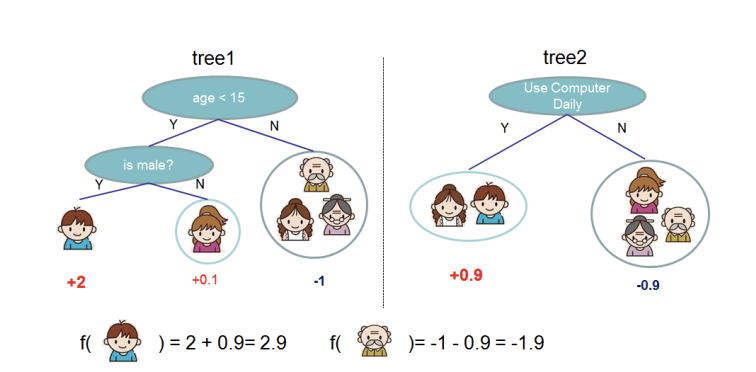
\includegraphics[width=0.8\textwidth]{xgboost_ensemble.png}
  \caption{XGBoost ensemble.}
  \label{xgboost-ensemble}
\end{figure}

\subsection{XGBoost Splitting Algorithm}

Here is a quick summary of XGBoost's splitting algorithm based on its original paper [1].
Let dataset $\mathcal{D} = \left\{ (\mathbf{x}_i, y_i) \right\}$ with $|\mathcal{D}| = n$, $\mathbf{x}_i \in \R^m$, and $y_i \in \R$.
The prediction is given by 
\begin{equation*}
  \hat{y}_i = \phi(\mathbf{x}_i) = \sum_{k=1}^K f_k(\mathbf{x}_i), \quad f_k \in \mathcal{F},
\end{equation*}

where $\mathcal{F}$ is the space of all possible trees. Each $f(\mathbf{x})$ maps an input feature vector to a leaf node label, which is a constant.
Notate this as $f(x) = w_{q(x)}$, where $q: \R^m \to T$, $w \in \R^T$, and $T$ is the number of leaves.
The loss function is given by a regularized objective which aims to minimize the loss and the complexity of the model, given by
\begin{equation*}
  \mathcal{L} = \sum_{i=1}^n l(y_i, \hat{y}_i) + \sum_{k=1}^K \Omega(f_k), \quad \Omega(f) = \gamma T + \frac{1}{2} \lambda \sum_{j=1}^T w_j^2.
\end{equation*}

This is difficult to obtimize directly, so the model is trained additively. That is, one tree is trained at a time, and the next tree is trained to correct the residuals of sum of the previous trees.
The $t$-th tree is trained to minimize
\begin{equation*}
  \mathcal{L}^{(t)} = \sum_{i=1}^n l(y_i, \hat{y}_i^{(t-1)} + f_t(\mathbf{x}_i)) + \Omega(f_t) + \text{constant},
\end{equation*}

where the constant is because the previous trees are fixed. To further simplify, a second order approximation is used and constant terms are dropped, to form the approximate loss
\begin{equation*}
  \tilde{\mathcal{L}}^{(t)} = \sum_{i=1}^n \left[ g_i f_t(\mathbf{x}_i) + \frac{1}{2} h_i f_t^2(\mathbf{x}_i) \right] + \Omega(f_t),
\end{equation*}

where $g_i = \partial_{\hat{y}^{(t-1)}} l(y_i, \hat{y}^{(t-1)})$ and $h_i = \partial_{\hat{y}^{(t-1)}}^2 l(y_i, \hat{y}^{(t-1)})$.
Then, define $I_j = \left\{ i | q(\mathbf{x}_i) = j \right\}$, intuitively being the set of all data points that fall into leaf $j$. Then expanding the approximate loss, and rearranging summations,
\begin{equation*}
  \tilde{\mathcal{L}}^{(t)} = \sum_{j=1}^T \left[ \left( \sum_{i \in I_j} g_i \right) w_j + \frac{1}{2} \left( \sum_{i \in I_j} h_i + \lambda \right) w_j^2 \right] + \gamma T.
\end{equation*}

Considering a fixed structure $q$, the optimal leaf values $w_j$ can be found by setting the derivative of the loss to zero, giving
\begin{equation*}
  w_j^* = -\frac{\sum_{i \in I_j} g_i}{\sum_{i \in I_j} h_i + \lambda}, \quad \text{and} \quad \tilde{\mathcal{L}}^{(t)}(q) = -\frac{1}{2} \sum_{j=1}^T \frac{\left( \sum_{i \in I_j} g_i \right)^2}{\sum_{i \in I_j} h_i + \lambda} + \gamma T.
\end{equation*}

To find the best structure $q$, the algorithm starts from a single leaf node and greedily adds branches to all the leaves. The best split ($I_R$, $I_L$) of a leaf with instance set $I$ then minimizes
\begin{equation*}
  \mathcal{L}_\text{split} = \frac{1}{2} \left[ \frac{\left( \sum_{i \in I} g_i \right)^2}{\sum_{i \in I} h_i + \lambda} - \frac{\left( \sum_{i \in I_L} g_i \right)^2}{\sum_{i \in I_L} h_i + \lambda} - \frac{\left( \sum_{i \in I_R} g_i \right)^2}{\sum_{i \in I_R} h_i + \lambda} \right] - \gamma.
\end{equation*}

To find the best split exactly, one can sort the instances by feature and iterate through all possible splits. However, this will be computationally expensive for large datasets
Instead, XGBoost uses an approximate algorithm by searching over a representative subset of the data given by quantiles.

\subsection{XGBoost Limitations}

XGBoost has its limitations. Firstly, its greedy training structure may lead to suboptimal solutions.
Secondly, it uses axis-aligned trees which may limit expressiveness especially when features are correlated.
Lastly, it is a piecewise constant predictor, which may not be the best representation of the data. As an example
see Figure~\ref{piecewise-constant}, XGBoost's attempt to fit a linear function.

\begin{figure}
  \centering
  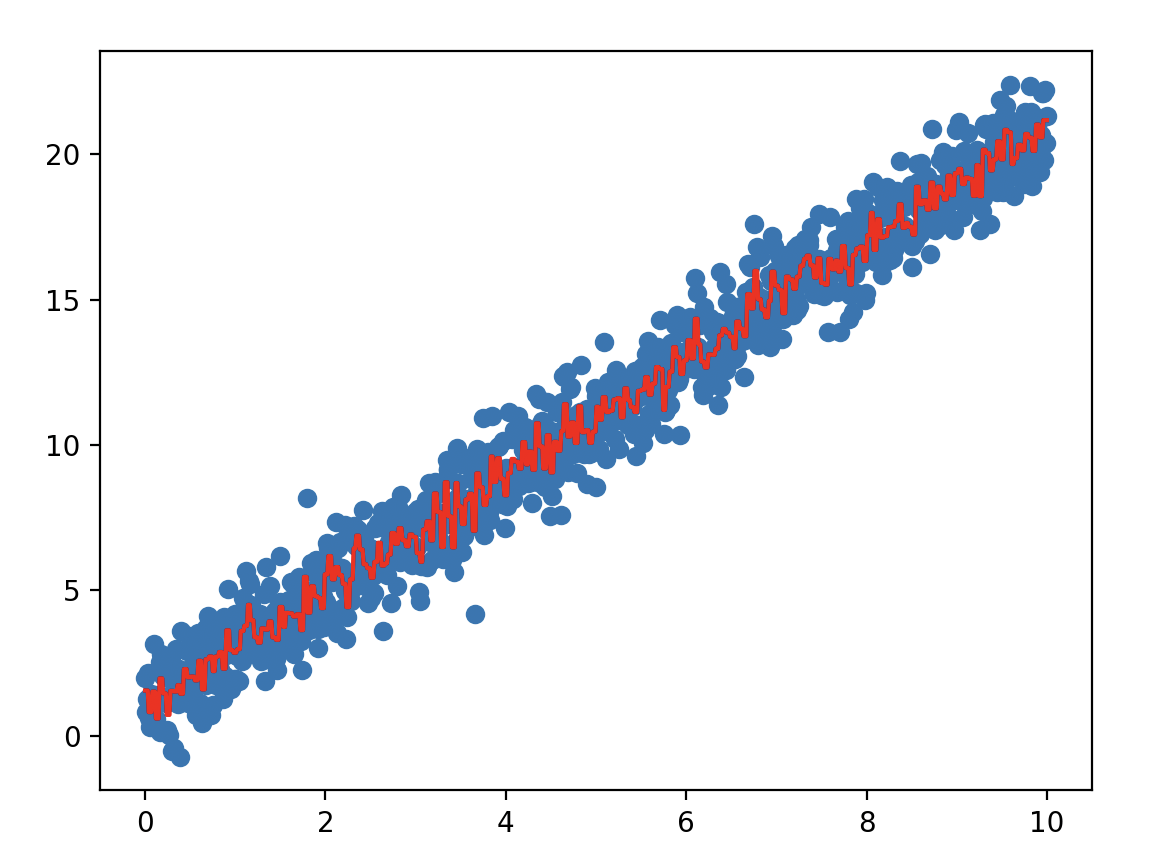
\includegraphics[width=0.8\textwidth]{piecewise_constant.png}
  \caption{XGBoost's attempt to fit a linear function.}
  \label{piecewise-constant}
\end{figure}

\section{Convex Tree Alternating Optimization}
Unlike XGBoost, tree alternating optimization (TAO) trains a single tree with oblique splits and modular leaf predictors (constant, linear, etc.) [2].
Here is a quick summary of the CTAO algorithm for $K$-class classification. Each non-leaf node in the tree is given by $\boldsymbol{\theta}_j = \left\{ \mathbf{w}_j, b_j \right\}$, where $\mathbf{w}_j \in \R^m$ and $b_j \in \R$.
An entering datapoint $\mathbf{x}$ is sent to the left child if $\mathbf{w}_j^T\mathbf{x} > b_j$ and to the right child otherwise. Each leaf node in the tree is given by $\theta_j \in \left\{ 1, \dots, K \right\}$.
Like XGBoost, predictions are made by the path from the root to the leaf, each intermediate node representing a decision. However, unlike XGBoost, only an individual, more powerful oblique tree is trained.

For classification, the leaf nodes gave a constant label. For regression problems, this can be simply adapted to create piecewise linear regression trees by having the leaf nodes give a linear prediction: 
$\theta_j = \left\{ \mathbf{w}_j, b_j \right\}$, where $\mathbf{w}_j \in \R^m$ and $b_j \in \R$, the prediction is given by $\mathbf{w}_{j}^T\mathbf{x} + b_{j}$.

Additionally, unlike XGBoost, the tree is not trained in a greedy fashion. Rather than a single leaf node, the tree is initialized randomly at a fixed depth, with random labels for leaf nodes and random splits for non-leaf nodes.
Then, the tree is trained by optimizing each individual node's parameters.

\subsection{TAO / CTAO Leaf Node Training Algorithm}

Consider a leaf node $j$. Based on the fixed tree structure and the decisions made above it, original dataset $\mathcal{D} = \left\{ (\mathbf{x}_i, y_i) \right\}$ with $|\mathcal{D}| = n$, $\mathbf{x}_i \in \R^m$, and $y_i \in \R$
is filtered to $\mathcal{D}_\text{seen}$, the subset of data points that reach the leaf node. It is then clear that for classification, the optimal label for the leaf node is the most common label in $\mathcal{D}_\text{seen}$,
\begin{equation*}
  \theta_j^* = \arg\max_{k} \sum_{(\mathbf{x}_i, y_i) \in \mathcal{D}_\text{seen}} \mathbb{I}(y_i = k),
\end{equation*}

For piecewise constant regression, the optimal label for the leaf node is the mean of the labels in $\mathcal{D}_\text{seen}$,
\begin{equation*}
  \theta_j^* = \frac{1}{|\mathcal{D}_\text{seen}|} \sum_{(\mathbf{x}_i, y_i) \in \mathcal{D}_\text{seen}} y_i.
\end{equation*}

For piecewise linear regression, the optimal label for the leaf node is the linear regression of the labels in $\mathcal{D}_\text{seen}$. This can be
found, for example, by solving a LASSO problem,
\begin{equation*}
  \theta_j^* = \arg\min_{\mathbf{w}_j, b_j} \sum_{(\mathbf{x}_i, y_i) \in \mathcal{D}_\text{seen}} \left( \mathbf{w}_j^T\mathbf{x}_i + b_j - y_i \right)^2 + \lambda \left\| \mathbf{w}_i \right\|_1.
\end{equation*}

\subsection{TAO / CTAO Non-Leaf Node Training Algorithm}

Consider a non-leaf node $i$. Based on the fixed tree structure and the decisions made above it, original dataset $\mathcal{D} = \left\{ (\mathbf{x}_i, y_i) \right\}$ with $|\mathcal{D}| = n$, $\mathbf{x}_i \in \R^m$, and $y_i \in \R$
is filtered to $\mathcal{D}_\text{seen}$, the subset of data points that reach the non-leaf node. Intuitively, it is the goal of this node to find the best split to separate the data points in $\mathcal{D}_\text{seen}$
so that the fixed tree structure below it can make the best decisions (properly classify or predict the data points).

For classification, there are three subsets of $\mathcal{D}_\text{seen}$ to consider. Firstly, the $(\mathbf{x}_i, y_i)$ where sending it left or right would both lead to the correct prediction.
Secondly, the $(\mathbf{x}_i, y_i)$ where sending it left or right would both lead to the incorrect prediction. 
Lastly, the $(\mathbf{x}_i, y_i)$ where sending it one way would lead to the correct prediction and sending it the other way would lead to the incorrect prediction. 
Let this be denoted by $\mathcal{D}_\text{care} \subseteq \mathcal{D}_\text{seen}$.

Intuitively, for the data $\mathcal{D}_\text{don't care} = \mathcal{D}_\text{seen} \setminus \mathcal{D}_\text{care}$, the fate of the datapoint is already decided by the fixed tree structure above and below this node,
and the decision of this node cannot change the correctness of the prediction. Therefore, only the set $\mathcal{D}_\text{care}$ is considered when finding the splitting hyperplane.

Let $X_\text{care} = \left\{ \mathbf{x}_i \right\}_{(\mathbf{x}_i, y_i) \in \mathcal{D}_\text{care}}$ and $\bar{y}_\text{care} = 1$ if $y_i$ is correctly predicted if $x_i$ is sent left and $-1$ if $y_i$ is correctly predicted if $x_i$ is sent right.
Then, the optimal hyperplane is found by minimizing the convex loss function,
\begin{equation*}
  \min_{\mathbf{w}_i, b_i} \sum\left(1-\bar{y} \odot\left(X_{\text {care }}^T w+b\right)\right),
\end{equation*}

where $\odot$ is the element-wise product. This is a convex optimization problem and can be solved efficiently, and it is easily interchangable with other convex loss functions for finding splitting hyperplanes.

Note that the original TAO algorithm [2] instead uses neural networks to split the data. However, the custom CTAO implementation uses the convex loss function above,
which can be easily solved with convex optimization techniques.

\subsection{Seperability of Nodes}

Following Theorem 3.1 in the original TAO paper [2], the nodes in the tree that are not descendants of eachother are separable.
As a result, to optimize the sum of losses over all the nodes in the TAO tree, it suffcces to optimize seperately over the parameters of any set of nodes 
that are not descendants of eachother. Further, this allows for parallelization of the optimization problem: nodes that are not descendants of eachother can be optimized in parallel.

The proof is very simple, as for two nodes $i$ and $j$ that are not descendants of eachother, their respective $\mathcal{D}_\text{seen}$ are disjoint. So, in minimizing 
the sum of all the losses over all the nodes in the tree, the loss of node $i$ is independent of the loss of node $j$. A formal proof is given in the original TAO paper [2].

\subsection{Difference Between TAO and CTAO}

There are two main differences between the original TAO algorithm and the custom CTAO algorithm. 
Firstly, as already noted, the original TAO algorithm uses neural networks to split the data at non-laef nodes, while the custom CTAO implementation uses the convex loss function. 
The CTAO implementation is more easily parallelizable and can be solved with convex optimization techniques.
Secondly, the original TAO algorithm, while proven to be parallelizable, did not have a parallelized implementation. The custom CTAO implementation is parallelized and can be run on multiple cores.
Both qualities make CTAO the first tree algorithm of its kind.


\section{CTAO Parallelization}

Since non-descendants are seperable, an easy way to parallelize the tree optimization problem is to optimize each layer of the tree in parellel.
From experimentation, the order in which the layers were optimized did not matter much, but the chosen order is a bottom-up approach, where the leaves are optimized first, then the nodes above the leaves, and so on.

Parallelization is done with Python Multiprocessing, enabling the use of multiple cores on a single machine. The number of cores used can be specified by the user.
To reduce the communication overhead of multiprocessing, the tree is serialized into a numpy array and with training data $X$ and $y$, is stored in shared memory for each process to access quickly.

\section{Results and Comparison with XGBoost}

The custom CTAO implementation and code to reproduce the results can be found at \url{https://github.com/albertcai101/convex-tree-alternating-optimizer}.

Unlike XGBoost which needs to train many trees, CTAO only needs to train a single tree. Additionally impressive is that CTAO's one-iteration performance is comparable with XGBoost.
That is, only one bottom-up layer by layer pass is needed to train the tree. As a result, for the default XGBoost configuration with $100$ trees of depth $6$, each tree must optimize
$2^7 - 1 = 127$ nodes, amounting to $12700$ optimization problems. In contrast, the CTAO implementation used in the results, which is $10$ layers deep, only needs to optimize
$2^{11} - 1 = 2047$ nodes. As a result, \emph{CTAO only needs to solve $16\%$ of the smaller optimization problems that XGBoost needs to solve}.

For preliminary results, only binary classification were tested, and extension to multi-class classification and regression is not expected to yield very different comparisons.
Three binary classification datasets were tested: the BACE-1 gene binding affinity dataset, the HIV detection from molecular structure dataset, and a subset of the SIDER side effect dataset
from molecular structure involving eye disorder dataset.

The results are shown in Tables~\ref{bace}, \ref{hiv}, and \ref{sider}. The results are promising, showing that CTAO is comparable with XGBoost, with CTAO beating XGBoost in one, and XGBoost beating CTAO in one.
For the HIV dataset, which is imbalanced both CTAO and XGBoost performed very poorly, not yielding any substantial comparision results.

\begin{table}[H]
  \centering
  \begin{tabular}{l r r c}
    \toprule
    \textbf{BACE} & \textbf{\% Accuracy} & \textbf{\% AUROC} \\
    \midrule
    XGB & $\boldsymbol{71\%}$ & $\boldsymbol{74\%}$ \\
    CTAO& {68\%} & {70\%} \\
    \bottomrule
  \end{tabular}
  \vspace{0.5cm}
  \caption{results of BACE-1 gene binding affinity classification.}
  \label{bace}
\end{table}

\begin{table}[H]
  \centering
  \begin{tabular}{l r r c}
    \toprule
    \textbf{HIV} & \textbf{\% Accuracy} & \textbf{\% AUROC} \\
    \midrule
    XGB & {98\%} & $\boldsymbol{59\%}$ \\
    CTAO& $\boldsymbol{98\%}$ & {50\%} \\
    \bottomrule
  \end{tabular}
  \vspace{0.5cm}
  \caption{results of HIV detection from molecular structure (imbalanced)}
  \label{hiv}
\end{table}

\begin{table}[H]
  \centering
  \begin{tabular}{l r r c}
    \toprule
    \textbf{SIDER} & \textbf{\% Accuracy} & \textbf{\% AUROC} \\
    \midrule
    XGB & {65\%} & {61\%} \\
    CTAO& $\boldsymbol{68\%}$ & $\boldsymbol{66\%}$ \\
    \bottomrule
  \end{tabular}
  \vspace{0.5cm}
  \caption{results of eye disorder detection from molecular structure (imbalanced)}
  \label{sider}
\end{table}

\medskip

\medskip

\medskip


{
\small


[1] Chen, T.\ and Guestrin, C.\ (2016) {\it XGBoost: A Scalable Tree Boosting System},

[2] Cerreira-Perpiñán, M.\ and Zharmagambetov, A.\ (2018) {\it Alternating Optimization of Decision Trees, with Application to Learning Sparse Oblique Trees.}

%%%%%%%%%%%%%%%%%%%%%%%%%%%%%%%%%%%%%%%%%%%%%%%%%%%%%%%%%%%%


\end{document}